\documentclass[11pt]{article}

\usepackage[margin=1in]{geometry}
\usepackage[T1]{fontenc}
\usepackage[utf8]{inputenc}
\usepackage{lmodern}
\usepackage{microtype}
\usepackage{amsmath,amssymb}
\usepackage{booktabs}
\usepackage{tabularx}
\usepackage{array}
\usepackage{enumitem}
\usepackage{xcolor}
\usepackage{tikz}
\usetikzlibrary{positioning,fit,arrows.meta,calc,backgrounds}
\usepackage{multirow}
\usepackage{caption}
\captionsetup[table]{skip=5pt}
\usepackage[round,authoryear]{natbib}
\usepackage[colorlinks=true,linkcolor=blue!50!black,citecolor=blue!50!black,urlcolor=blue!50!black]{hyperref}

\newcommand{\Lcal}{\mathcal{L}}
\newcommand{\sg}{\operatorname{sg}}
\newcommand{\SIGReg}{\operatorname{SIGReg}}
\newcolumntype{Y}{>{\raggedright\arraybackslash}X}
\setlist{itemsep=2pt,topsep=4pt}

\title{Hierarchical LLM-JEPA for Code:\\
Span-Grounded, Multi-Level Representation Learning\\
with Pretrained Code Language Models\\[0.5em]
\large Research proposal --- draft of \today}
\author{Code-JEPA project}
\date{}

\begin{document}
\maketitle

\begin{abstract}
We propose to train a pretrained code language model so that its internal representations of a program are
organised by level of abstraction: individual statement blocks (\emph{steps}), functions and methods (\emph{units}),
and the whole program, seen both as an algorithmic \emph{approach} (how) and as an \emph{intent} (what). The training
signal comes from a dataset of 111.5k test-verified Python programs, each annotated with a tree of natural-language
descriptions whose shape is extracted from the abstract syntax tree, so that every description is grounded in a
real code span. We treat each level's description as a separate \emph{view} of the program and apply a joint-embedding
predictive (JEPA) loss at every level of the tree, following the LLM-JEPA recipe for language models and the
H-JEPA recipe for hierarchies of latent spaces. A single pretrained model encodes code and descriptions and also
acts as the predictor; the hierarchy is implemented inside the model through one special token per tree node and
a tree-shaped attention mask. A next-token loss anchors the backbone, and a per-level isotropic-Gaussian regulariser
(SIGReg) protects the new node embeddings from collapse. We describe the data, the architecture, the losses, the
experiments and controls, and the evaluation, with emphasis on showing that the learned levels are distinct and
individually useful rather than redundant copies of program meaning. First results with a 0.5B backbone on
CodeContests (three seeds) support the hypothesis: the hierarchical model is the only one whose frozen
representations encode step- and function-level descriptions beyond the pretrained model, flat LLM-JEPA strongly
improves program-level alignment, and neither hurts the next-token loss. The diagnostics that led to the training
recipe (no stop-gradient, a small SIGReg memory bank and per-level SIGReg weights) are reported in full.
\end{abstract}

% ===========================================================================
\section{Introduction}
% ===========================================================================

Programs have an explicit hierarchy: tokens form statements, statements form blocks, blocks form functions, and
functions combine into a program that implements an algorithm for a task. Code models are usually trained on flat
token sequences with next-token prediction, and code embedding models usually produce one vector per snippet. Neither
is asked to represent a program at several levels of abstraction at once, and neither is told which spans of code
correspond to which level.

Joint-embedding predictive architectures (JEPAs) learn by predicting the \emph{representation} of one view of the data
from another, rather than reconstructing inputs \citep{lecun2022path,assran2023ijepa}. Two recent lines of work make
this directly applicable to our setting. LLM-JEPA \citep{huang2025llmjepa} shows that adding a JEPA loss between two
views of the same sample (for example, a natural-language request and the corresponding code) to the usual
next-token loss improves fine-tuned language models. H-JEPA \citep{zhang2026hjepa}, which implements the
hierarchical JEPA proposed by \citet{lecun2022path}, shows how to train a stack of JEPAs end-to-end, each level with
its own encoder, predictor and latent space, without collapse.

Our collaborator has built a dataset designed for exactly this combination: every program comes with descriptions at
four levels (intent, approach, unit, step), each tied to an AST span, so that each level is a separate view of the
same program. This proposal describes how we will use it.

\paragraph{Hypothesis.}
\emph{Training a pretrained code language model with a JEPA loss at every level of a span-grounded description tree,
anchored by the next-token loss, produces representations whose levels are distinct and individually useful, and
improves description-to-code generation and code understanding over regular fine-tuning and flat LLM-JEPA.}

\paragraph{Contributions (planned).}
\begin{enumerate}
  \item A hierarchical extension of LLM-JEPA in which one JEPA loss is applied per node of a program's description
        tree, with the hierarchy implemented inside a pretrained model by node tokens and a tree attention mask.
  \item A transfer of the H-JEPA training recipe (per-level predictors and losses, SIGReg, no EMA or
        stop-gradient) from temporal world models to the structural hierarchy of programs.
  \item An evaluation protocol that tests level distinctness directly (level-confusion matrices, per-level rank,
        controls for the amount of supervision), alongside generation pass@1 and retrieval.
\end{enumerate}

% ===========================================================================
\section{Related work and the principles we adopt}
\label{sec:related}
% ===========================================================================

This section acknowledges the work our design draws on and states, for each, which principle we adopt and where it
appears in our method. Table~\ref{tab:principles} summarises the mapping.

\subsection{JEPA foundations}

\paragraph{A path towards autonomous machine intelligence \citep{lecun2022path}.}
This position paper introduces JEPAs and the hierarchical JEPA (H-JEPA): a stack of JEPAs in which each level
encodes the representations of the level below, and higher levels are more abstract and predict over longer ranges.
It argues for prediction in representation space rather than input space, and for preventing collapse through
regularisation rather than only contrastive negatives.
\emph{Adopted:} prediction in representation space, and the idea that each level encodes the representations of the
level below. In our case the levels are structural (step $\to$ unit $\to$ program) rather than temporal.

\paragraph{I-JEPA \citep{assran2023ijepa} and V-JEPA \citep{bardes2024vjepa}.}
These works instantiate JEPAs for images and video: a context encoder sees a partially masked input, and a predictor,
conditioned on the position of the hidden region, predicts the target encoder's representation of that region.
\emph{Adopted:} masked-region prediction conditioned on the target's position. We use AST nodes as the masked regions
in an auxiliary, code-only objective (Section~\ref{sec:loss-mask}). We do not adopt their EMA target encoder (see
H-JEPA below).

\paragraph{VICReg \citep{bardes2022vicreg} and LeJEPA / SIGReg \citep{balestriero2025lejepa}.}
VICReg prevents collapse with explicit variance and covariance penalties on embeddings. LeJEPA replaces such
heuristics with SIGReg, a sketched test that pushes the embedding distribution towards an isotropic Gaussian along
random projections.
\emph{Adopted:} SIGReg, applied per level to the node embeddings (Section~\ref{sec:loss-dist}). VICReg-style
penalties remain an alternative.

\subsection{LLM-JEPA}

\paragraph{LLM-JEPA \citep{huang2025llmjepa}.}
LLM-JEPA adds a JEPA term to language-model fine-tuning on datasets that have two views of the same content, such as
a natural-language request and its regular expression, SQL query or worked solution. From the paper and its
reference implementation we take the following elements:
\begin{itemize}
  \item \textbf{One shared encoder.} The language model itself embeds both views; the embedding of a view is the
        last-layer hidden state at its last token. There is no EMA target and no stop-gradient.
  \item \textbf{The model is also the predictor.} A few special predictor tokens are appended to the first view,
        and the hidden state of the last one is the prediction; the predictor shares all weights with the encoder.
  \item \textbf{Loss.} $\gamma\,\Lcal_{\text{LM}} + \lambda\,\bigl(1-\cos(\mathrm{Pred}(\mathrm{Enc}(\text{Text})),
        \mathrm{Enc}(\text{Code}))\bigr)$, where the next-token loss $\Lcal_{\text{LM}}$ keeps the representations
        informative and is what prevents collapse.
  \item \textbf{Practical recipe.} 1--2B-parameter models, learning rate $10^{-5}$, four epochs, $\lambda\in\{0.5,2\}$,
        zero to two predictor tokens, several seeds; packing both views into one row with a block-diagonal 4D
        attention mask; random JEPA-loss dropout to reduce compute; and comparisons with regular fine-tuning at equal
        FLOPs.
\end{itemize}
\emph{Adopted:} all of the above, as the core of our method. Our extension is to apply the JEPA loss once per node of
a description tree instead of once per sample (Sections~\ref{sec:arch} and~\ref{sec:losses}). We also take from its
ablations the alternatives we compare against: L2, MSE and InfoNCE distances, and the reversed prediction direction.

\paragraph{Semantic Tube Prediction \citep{llmjepa2025stp}.}
Released in the same repository, this variant embeds a span inside a sequence as the difference of hidden states at
its boundaries, and asks a span to be predictable from the rest of the sequence.
\emph{Adopted only as an ablation:} the boundary-difference span embedding. Because such differences telescope (a
parent span's difference is the sum of its children's), a hierarchy built on them would be trivially additive, so it
is not our main design.

\subsection{Hierarchical JEPAs}

\paragraph{H-JEPA \citep{zhang2026hjepa}.}
H-JEPA trains a hierarchy of action-conditioned JEPA world models end-to-end for visual planning. It builds on
LeWorldModel \citep{maes2026leworldmodel}, uses LeJEPA's SIGReg at every level, and releases its code. Its recipe
and findings shape several of our choices:
\begin{itemize}
  \item \textbf{Each level has its own encoder, predictor and latent space}, and each upper-level encoder reads the
        lower level's embeddings, not the raw input. Its window encoder pools a variable-length set of lower-level
        embeddings into one vector with a summary token and a padding mask.
        \emph{Adopted:} our node tokens read the tokens or nodes one level below; the window encoder is reused in our
        pooling-head ablation.
  \item \textbf{A loss per level, summed, trained end-to-end:} $\Lcal^{(\ell)}=\Lcal^{(\ell)}_{\text{pred}}+
        \lambda_\ell\SIGReg(Z^{(\ell)})$, with gradients from upper levels flowing into lower encoders, no EMA and
        no stop-gradient. \emph{Adopted:} level-specific predictors and per-level loss weights, SIGReg on every
        level, and no stop-gradient by default.
  \item \textbf{SIGReg, not target detachment, prevents collapse.} Without SIGReg, the embeddings collapsed to an
        effective rank of 1--14 out of 384 whether or not targets were detached. \emph{Adopted:} our new node tokens
        are not shaped by the next-token loss, so we regularise them with SIGReg and monitor per-level rank.
  \item \textbf{Slow-feature collapse is an optimum of the prediction loss}, which no regulariser on the marginal
        distribution can exclude (building on \citet{sobal2022slow}); H-JEPA needed grounded supervision (an
        inverse-dynamics head) to retain task-relevant information. \emph{Adopted:} our description views serve as
        that grounding, and code-only prediction is never used without them.
  \item \textbf{An upper level helps only when the data has structure at that scale}, and stagewise training lets
        each level train on suitable data. \emph{Adopted:} we report unit-level results separately for multi-unit
        programs and include stagewise training as an ablation.
  \item \textbf{The ``HWM'' baseline} uses identity upper-level encoders. \emph{Adopted:} as a control in which a
        parent's vector is the mean of its children's.
  \item \textbf{Per-level learning rates.} \emph{Adopted:} a higher rate for newly introduced parameters than for the
        pretrained backbone.
\end{itemize}
H-JEPA lists variable-duration segments and alignment of upper-level latents with language as future work; our AST
spans and level-wise descriptions provide both.

\subsection{Hierarchical latent prediction in language models}

\paragraph{HiLP \citep{shi2026hilp} and NextLat \citep{teoh2025nextlat}.}
NextLat adds a next-latent prediction loss to language-model pretraining. HiLP extends it with a second level: a
sliding-window module summarises the last $k=4$ token states, and an upper predictor forecasts that summary $k$
tokens ahead, with stop-gradient targets. A combined head predicts the next token from both levels. The hierarchy is
removed at inference; the goal is better next-token prediction (HumanEval pass@1 rises from 8.8 to 11.3 for 1B models
trained on 100B tokens).
\emph{Relation to our work:} closely related in spirit but a different method. HiLP's levels are fixed token windows
learned without supervision during pretraining, and the levels are not evaluated as representations. Ours are AST
spans with a description at each level, built on a pretrained model, and the level-wise representations are the
object of study. Its combined head, which gives the upper level a next-token training signal, is a candidate way to
anchor our node tokens generatively (an ablation alongside SIGReg).

\paragraph{Next-Concept Modeling \citep{kumbong2026ncm}.}
NCM is a fast, non-autoregressive text generator. A multiscale residual VQ-VAE encodes text into $K$ levels of
discrete codes, from a few coarse codes to one per token, each level encoding the residual left by the coarser ones.
A transformer, trained from scratch, then generates the levels coarse to fine, predicting all codes of a level in
parallel. Its levels are resolution levels with fixed lengths and no attached meaning, and it does not use JEPA
objectives or evaluate on code, so it is a different method with a different goal.
\emph{Adopted:} two ideas. First, \emph{nested dropout}: the tokenizer is trained on reconstructions from a random
number of coarse levels, so that coarse levels must carry useful information on their own. Our analogue is to
condition the next-token loss on a random prefix of the description levels (intent; plus approach; plus units; plus
steps), which we evaluate against the fixed intent-and-approach prompt. Second, its \emph{intervention probes}: fixing
coarse codes and resampling fine ones, mixing the coarse codes of two inputs, and perturbing a few coarse codes,
then inspecting what changes in the output. We adapt these to programs when generation is conditioned on our node
embeddings (Section~\ref{sec:evaluation}). Its residual coding, which makes levels non-redundant by construction,
motivates a residual parameterisation of child nodes as an ablation. Like H-JEPA and HiLP, NCM lists an
input-dependent hierarchy as future work; our AST-derived trees provide one.

\subsection{Code representation learning and contrastive alignment}

Contrastive objectives \citep{oord2018cpc}, popularised for paired modalities by CLIP \citep{radford2021clip}, and
code embedding models such as UniXcoder \citep{guo2022unixcoder} and CodeSage \citep{zhang2024codesage} learn one
vector per snippet. Our earlier design for this project followed this pattern, with a code encoder aligned to a frozen
text-embedding model such as BGE \citep{xiao2023cpack}. We keep it as a baseline (B1) and keep InfoNCE with
other-level hard negatives as an alternative distance.

\begin{table}[t]
\centering
\small
\caption{Principles adopted from prior work and where they appear in our method.}
\label{tab:principles}
\begin{tabularx}{\textwidth}{@{}p{3.2cm}YY@{}}
\toprule
Work & Principle adopted & Where in our method \\
\midrule
\citet{lecun2022path} & Predict in representation space; each level encodes the level below & All JEPA losses; node tokens read the level below (\S\ref{sec:arch}) \\
\citet{assran2023ijepa,bardes2024vjepa} & Masked-region prediction conditioned on the target's position & Masked-node objective (\S\ref{sec:loss-mask}) \\
\citet{huang2025llmjepa} & One shared LM encoder and predictor; predictor tokens; LM loss + cosine JEPA loss; packing, loss dropout, equal-FLOP comparison & Core objective (\S\ref{sec:loss-view}), packing (\S\ref{sec:packing}), protocol (\S\ref{sec:experiments}) \\
\citet{llmjepa2025stp} & Boundary-difference span embedding & Ablation only \\
\citet{zhang2026hjepa} & Per-level encoder, predictor and loss; end-to-end, no EMA; SIGReg per level; grounding against slow features; HWM and stagewise controls & Node hierarchy, losses (\S\ref{sec:loss-dist}), controls (\S\ref{sec:experiments}) \\
\citet{balestriero2025lejepa} & SIGReg & Per-level anti-collapse term \\
\citet{sobal2022slow} & JEPAs favour slow, easy-to-predict features & Masked-node objective is always combined with description views \\
\citet{shi2026hilp} & Combined head that anchors the upper level with next-token loss & Ablation for anchoring node tokens \\
\citet{kumbong2026ncm} & Nested dropout over levels; intervention probes on coarse levels; residual coding & Random prompt depth (\S\ref{sec:loss-anchor}); intervention probes (\S\ref{sec:evaluation}); residual ablation \\
\citet{oord2018cpc,radford2021clip} & Contrastive alignment with in-batch negatives & InfoNCE distance option; baseline B1 \\
\bottomrule
\end{tabularx}
\end{table}

% ===========================================================================
\section{Data}
\label{sec:data}
% ===========================================================================

\paragraph{Sources.}
The dataset was built by our collaborator from three sources of test-verified Python solutions:
CodeContests \citep{li2022alphacode} (11,677 programs, stdio tests, up to two solutions per problem),
TACO \citep{li2023taco} (25,181 programs) and a 100k subsample of KodCode-V1 \citep{xu2025kodcode} (74,667
function-level programs with pytest tests), 111.5k programs in total. All solutions pass their tests, and the data is
decontaminated against HumanEval+ and MBPP+ \citep{chen2021humaneval,liu2023evalplus} and the TACO and CodeContests
evaluation splits. KodCode's licence restricts the combined data to non-commercial research.

\paragraph{The description tree.}
The shape of each tree is extracted deterministically with tree-sitter \citep{treesitter}; a teacher LLM then writes
one description per node, bottom-up, in a single guided-JSON call. The levels are listed in
Table~\ref{tab:levels}. Each level must be strictly more abstract than the one below it, and descriptions follow what
the code does rather than the problem statement.

\begin{table}[t]
\centering
\small
\caption{Levels of the description tree. Every description is tied to an AST span.}
\label{tab:levels}
\begin{tabularx}{\textwidth}{@{}lYl@{}}
\toprule
Level & Description & Span \\
\midrule
Intent & What problem is solved; must hold for any correct solution & whole program \\
Approach & Algorithmic strategy, key data structures, time and space complexity & whole program \\
Unit & Responsibility and contract (inputs, outputs, edge cases) & function, class, method, or \texttt{main} \\
Step & One line of pseudocode with key conditions and formulas; long blocks get child steps & AST block \\
Code & The verified solution & tokens \\
\bottomrule
\end{tabularx}
\end{table}

\subsection{Measured properties that constrain the design}
\label{sec:data-constraints}
The numbers in Table~\ref{tab:data-stats} were measured on the full annotation of each source. They rule out several
otherwise natural designs and dictate how we encode the tree, how we weight the losses, and how we interpret the
results.

\begin{table}[t]
\centering
\small
\caption{Tree shape and length, measured on the full annotation. Node counts include steps, units, and the two
program-level nodes. CC is CodeContests. Token estimates are from word and character counts and will be replaced by
tokenizer lengths in the loader.}
\label{tab:data-stats}
\begin{tabularx}{\textwidth}{@{}lYYYY@{}}
\toprule
& CC & TACO & KodCode & Design consequence \\
\midrule
Programs & 11{,}677 & 25{,}181 & 74{,}667 & \\
Nodes / program (median / p90 / p99 / max)
  & 8 / 21 / 46 / 81 & 7 / 17 / 42 / 76 & 7 / 13 / 25 / 67
  & Variable-size node set; no fixed latent slots \\
Single-unit programs
  & 63\% & 65\% & 74\%
  & Unit and program usually share a span \\
One unit and one step
  & 12\% & 21\% & 16\%
  & Three levels share a span; only the text differs \\
Units with a single top-level step
  & 39\% & 40\% & 37\%
  & Step and unit often share a span \\
Programs with nested steps
  & 29\% & 23\% & 10\%
  & Depth at most 2; parent steps exist \\
All descriptions, words (median / p99)
  & 235 / 911 & 209 / 862 & 172 / 550
  & $\approx$330 / 1{,}300 tokens of text views \\
Code, characters (median / p99)
  & 454 / 3{,}741 & 387 / 3{,}297 & 624 / 2{,}275
  & $\approx$150 / 1{,}100 code tokens \\
\bottomrule
\end{tabularx}
\end{table}

\paragraph{Variable-size trees, not a fixed latent budget.}
The number of nodes per program ranges from a handful to 81. A design with a fixed number of queries per level
(for example 16 steps, 4 units, 1 program) would either waste slots on typical programs or truncate the long tail.
We therefore allocate one token per node, cap at 96 nodes, and pad within a batch. Because node counts vary, the
view loss is averaged per node within each level so that large programs do not dominate the gradient.

\paragraph{Most programs are a single unit.}
In 63--74\% of programs the unit and the program describe the same span of code. In 12--21\% there is also only one
step, so intent, approach, unit and step all cover the same lines and differ only in wording (task, strategy,
contract, pseudocode). This is the central threat to the hypothesis: without extra pressure, the four embeddings can
collapse to one program vector. We therefore (i)~give approach and intent separate tokens rather than two heads on
one vector, and use each as a hard negative for the other; (ii)~report retrieval, confusion and probes separately
for single-unit and multi-unit programs, so that gains on the minority of multi-unit programs are not hidden;
(iii)~run masked-unit prediction only when there are at least two units, otherwise the context of the masked node
is empty; (iv)~include an HWM-style control in which a parent is the mean of its children, and a residual ablation
in which a child's embedding is its parent's plus a learned offset. H-JEPA's finding that an upper level helps only
when the data has structure at that scale \citep{zhang2026hjepa} is the reason for this split.

\paragraph{Steps almost partition units, and nest at most twice.}
About 39\% of units have a single top-level step, so those two descriptions share a span. We keep both targets but
log their embedding similarity separately, so that easy alignment on paraphrases of the same block is not counted as
evidence of a hierarchy. Compound statements of 14 lines or more receive child steps; a parent step summarises its
children, and no program has more than two levels of steps. The tree mask therefore has a parent-step token that
reads child-step tokens, with an option to flatten depth~2 into depth~1. Steps cover each unit's own executable
lines: uncovered lines are headers, blanks, comments, docstrings, imports, or lines of a nested unit, and are
assigned to that unit. Units themselves nest (\texttt{main} surrounds module-level code; classes contain methods),
and each line belongs to its innermost unit. The mask follows this nesting rather than treating units as a flat list.

\paragraph{Approach and intent are two views of one span.}
Both are written for the whole program. They are not two scales, so they must not share a code-side target: a single
program vector pulled toward both ``what'' and ``how'' would mix the two. Two tokens with the same mask, two
predictor heads, and mutual hard negatives are the corresponding design.

\paragraph{Several solutions share a problem.}
In CodeContests, 4{,}953 of 6{,}338 problems have two solutions; after merging with TACO, a cluster can have up to
four. Their intent texts describe the same task (identical wording in only about 5\% of pairs) while the approaches
may differ. Same-problem pairs are therefore masked as negatives in the contrastive option, and they supply
(i)~a code-to-code view for cross-solution intent prediction, (ii)~a free evaluation of solution-to-solution
retrieval, and (iii)~the swap probe in which two approaches to the same task are exchanged.

\paragraph{The packed sequence fits, and the text views are short.}
Median description lengths are 28 words (intent), 41 (approach), 36 (unit) and 18 (step). Code plus all descriptions
is about 550 tokens at the median and 2{,}600 at the 99th percentile of CodeContests, so a 3{,}072-token cap on the
view row should drop well under 1\% of programs (to be confirmed with the Qwen tokenizer). Length-bucketed batches
keep the 4D mask tractable. The LM row is shorter still: the default prompt is only intent and approach.

\paragraph{Intent is not a function of the code.}
The intent is written from the problem statement and must hold for any correct solution. It names objects
(``jumps'', ``tags'', ``phone numbers'') that need not appear in the identifiers. Low intent-level retrieval or
generation from intent alone is therefore not evidence that the hierarchy failed; the reconstruction study already
shows the floor (intent alone rewrites to passing code in 12\% of CodeContests samples versus 48\% of KodCode).
Generation pass@1 is reported by source and by prompt depth for this reason.

\paragraph{Every program has tests.}
All solutions were verified before annotation. The tests give a generation metric (pass@1 against the record's
harness) that does not depend on matching the teacher's phrasing, which in-distribution retrieval otherwise
rewards.

\paragraph{Splits and quality signals.}
5,034 of 6,365 CodeContests problems also appear in TACO under different identifiers, so we cluster problems by
normalised statement across sources and split by cluster (2--3\% for test). Soft quality flags (about 5\% of
records) can be used for filtering or down-weighting. In a reconstruction test on 200 samples, the teacher's pass
rate when rewriting code from the descriptions rises from 30.5\% (intent only) to 65.0\% (all levels).

% ===========================================================================
\section{Method}
\label{sec:arch}
% ===========================================================================

Figure~\ref{fig:arch} summarises the method. A single pretrained code model processes two packed rows per program.
The \emph{view row} carries the code followed by one special token per tree node, under a tree-shaped attention
mask, and then every description segment followed by its level's predictor token. The \emph{LM row} carries the
intent and approach as a prompt followed by the code. The node tokens give the code-side embeddings $c_v$ and the
predictor tokens give the description-side predictions $p_v$, both through per-level projection heads. The losses
are a per-node view loss between $p_v$ and $c_v$, a per-level SIGReg on both sides, and the next-token loss on the
LM row. No stop-gradient and no EMA target are used (Section~\ref{sec:exp-diag}).

\begin{figure}[t]
\centering
\resizebox{\textwidth}{!}{%
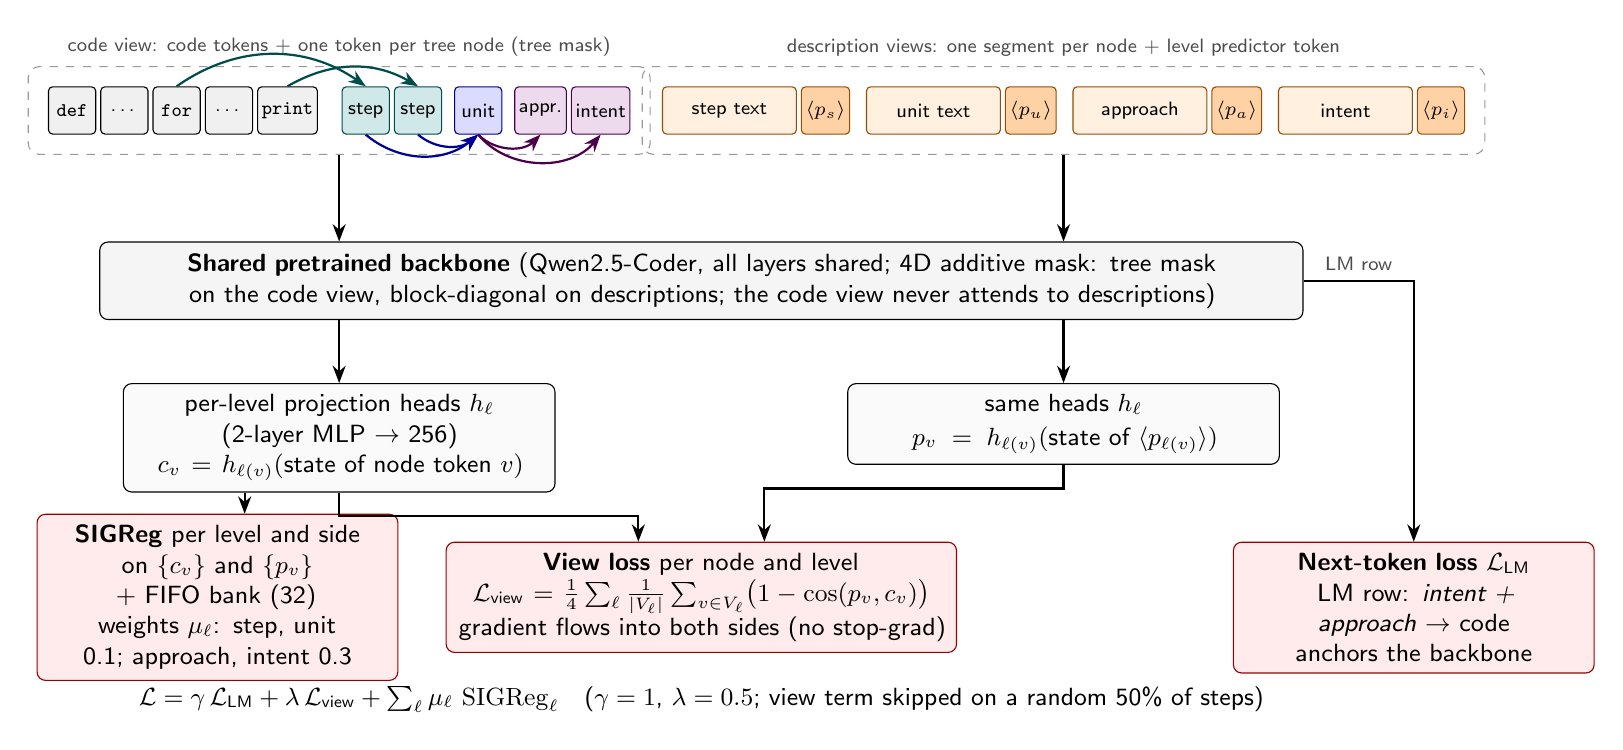
\begin{tikzpicture}[
    font=\sffamily\small,
    >={Stealth[length=2.2mm]},
    tok/.style={draw, rounded corners=1.5pt, minimum height=6mm, minimum width=6mm, inner sep=1.5pt, font=\sffamily\scriptsize},
    code/.style={tok, fill=gray!12},
    stepn/.style={tok, fill=teal!18, draw=teal!60!black},
    unitn/.style={tok, fill=blue!14, draw=blue!60!black},
    progn/.style={tok, fill=violet!14, draw=violet!60!black},
    desc/.style={tok, fill=orange!12, draw=orange!60!black, minimum width=17mm},
    pred/.style={tok, fill=orange!35, draw=orange!60!black},
    block/.style={draw, rounded corners=3pt, align=center, inner sep=4pt},
    loss/.style={block, fill=red!8, draw=red!60!black, font=\sffamily\small},
    lbl/.style={font=\sffamily\scriptsize, text=black!70, align=center},
  ]
  % ---------------- view row: code + node tokens ----------------
  \node[code] (c1) {\texttt{def}};
  \node[code, right=0.5mm of c1] (c2) {\dots};
  \node[code, right=0.5mm of c2] (c3) {\texttt{for}};
  \node[code, right=0.5mm of c3] (c4) {\dots};
  \node[code, right=0.5mm of c4] (c5) {\texttt{print}};
  \node[stepn, right=3mm of c5] (s1) {step};
  \node[stepn, right=0.5mm of s1] (s2) {step};
  \node[unitn, right=1.5mm of s2] (u1) {unit};
  \node[progn, right=1.5mm of u1] (ap) {appr.};
  \node[progn, right=0.5mm of ap] (in) {intent};
  % descriptions
  \node[desc, right=4mm of in] (d1) {step text};
  \node[pred, right=0.5mm of d1] (q1) {$\langle p_s\rangle$};
  \node[desc, right=2mm of q1] (d2) {unit text};
  \node[pred, right=0.5mm of d2] (q2) {$\langle p_u\rangle$};
  \node[desc, right=2mm of q2] (d3) {approach};
  \node[pred, right=0.5mm of d3] (q3) {$\langle p_a\rangle$};
  \node[desc, right=2mm of q3] (d4) {intent};
  \node[pred, right=0.5mm of d4] (q4) {$\langle p_i\rangle$};

  \begin{scope}[on background layer]
    \node[draw=black!40, dashed, rounded corners, fit=(c1)(in), inner sep=2.5mm, label={[lbl]above:code view: code tokens + one token per tree node (tree mask)}] (codebox) {};
    \node[draw=black!40, dashed, rounded corners, fit=(d1)(q4), inner sep=2.5mm, label={[lbl]above:description views: one segment per node + level predictor token}] (descbox) {};
  \end{scope}

  % tree-mask arrows ("reads")
  \draw[->, teal!60!black, thick] (c3.north) to[bend left=35] (s1.north);
  \draw[->, teal!60!black, thick] (c5.north) to[bend left=30] (s2.north);
  \draw[->, blue!60!black, thick] (s1.south) to[bend right=40] (u1.south);
  \draw[->, blue!60!black, thick] (s2.south) to[bend right=40] (u1.south);
  \draw[->, violet!60!black, thick] (u1.south) to[bend right=45] (ap.south);
  \draw[->, violet!60!black, thick] (u1.south) to[bend right=50] (in.south);

  % ---------------- shared backbone ----------------
  \node[block, fill=gray!8, minimum height=9mm, below=11mm of $(codebox.south)!0.5!(descbox.south)$,
        minimum width=0.98\linewidth, text width=15cm] (bb)
        {\textbf{Shared pretrained backbone} (Qwen2.5-Coder, all layers shared; 4D additive mask: tree mask on the code view,
         block-diagonal on descriptions; the code view never attends to descriptions)};
  \draw[->, thick] (codebox.south) -- (codebox.south |- bb.north);
  \draw[->, thick] (descbox.south) -- (descbox.south |- bb.north);

  % ---------------- heads ----------------
  \node[block, fill=gray!4, below=8mm of bb.south -| codebox.south, text width=5.2cm] (hc)
        {per-level projection heads $h_\ell$\\ (2-layer MLP $\to$ 256)\\ $c_v = h_{\ell(v)}(\text{state of node token } v)$};
  \node[block, fill=gray!4, below=8mm of bb.south -| descbox.south, text width=5.2cm] (hp)
        {same heads $h_\ell$\\[1pt] $p_v = h_{\ell(v)}(\text{state of } \langle p_{\ell(v)}\rangle)$};
  \draw[->, thick] (bb.south -| hc.north) -- (hc.north);
  \draw[->, thick] (bb.south -| hp.north) -- (hp.north);

  % ---------------- losses ----------------
  \node[loss, below=8mm of $(hc.south)!0.5!(hp.south)$, text width=6.2cm] (lv)
        {\textbf{View loss} per node and level\\ $\Lcal_{\text{view}} = \tfrac{1}{4}\sum_\ell \tfrac{1}{|V_\ell|}\sum_{v\in V_\ell}\bigl(1-\cos(p_v, c_v)\bigr)$\\
         gradient flows into both sides (no stop-grad)};
  \node[loss, left=6mm of lv, text width=4.3cm] (sr)
        {\textbf{SIGReg} per level and side\\ on $\{c_v\}$ and $\{p_v\}$ + FIFO bank (32)\\ weights $\mu_\ell$: step, unit 0.1; approach, intent 0.3};
  \coordinate (lmx) at ($(bb.east)+(14mm,0)$);
  \node[loss, anchor=north, text width=4.3cm] (lm) at (lmx |- lv.north)
        {\textbf{Next-token loss} $\Lcal_{\text{LM}}$\\ LM row: \textit{intent + approach} $\to$ code\\ anchors the backbone};
  \draw[->, thick] (hc.south) -- ++(0,-3mm) -| ([xshift=-8mm]lv.north);
  \draw[->, thick] (hp.south) -- ++(0,-3mm) -| ([xshift=8mm]lv.north);
  \coordinate (hcs) at ([xshift=-12mm]hc.south);
  \draw[->, thick] (hcs) -- (hcs |- sr.north);
  \draw[->, thick] (bb.east) -- ++(14mm,0) node[lbl, pos=0.5, above] {LM row} -- (lm.north);

  \node[below=3mm of lv, font=\sffamily\small] (tot)
        {$\Lcal = \gamma\,\Lcal_{\text{LM}} + \lambda\,\Lcal_{\text{view}} + \textstyle\sum_\ell \mu_\ell\,\SIGReg_\ell$\quad
         ($\gamma=1$, $\lambda=0.5$; view term skipped on a random 50\% of steps)};
\end{tikzpicture}}
\caption{Code-JEPA block diagram. Each program is packed into a view row and an LM row and processed by one shared
pretrained model. Arrows above the code view show the tree mask: a leaf step token reads its span's code tokens, a
unit token reads its step tokens, and the approach and intent tokens read the unit tokens (in the
\emph{free-program-token} variant they read all code tokens instead; Section~\ref{sec:exp-controls}). Node tokens give
code-side embeddings $c_v$; each description is followed by a level-specific predictor token whose state gives the
prediction $p_v$. A per-node cosine view loss aligns $p_v$ with $c_v$ at every level, SIGReg keeps each level's
embeddings spread, and a next-token loss on the LM row anchors the backbone.}
\label{fig:arch}
\end{figure}

\subsection{Backbone}
We fine-tune Qwen2.5-Coder \citep{hui2024qwen25coder}: the 0.5B model for development and the 1.5B base model as
the main backbone. This is the size range validated by LLM-JEPA, and full fine-tuning fits on a single 46\,GB GPU.
With about 111k programs and one million supervised nodes, our data is larger than the fine-tuning sets used by
LLM-JEPA. A 7B model with LoRA is an optional upper bound.

\subsection{Code view: node tokens with a tree attention mask}
After the code tokens we append one special token per node of the tree, in bottom-up order. A 4D attention mask,
applied at every layer, restricts what each token sees:
\begin{itemize}
  \item code tokens use normal causal attention over earlier code tokens;
  \item a leaf step token sees the code tokens in its lines;
  \item a parent step token sees its own header tokens and its child step tokens;
  \item a unit token sees its header, docstring and import tokens, its top-level step tokens, and nested unit tokens;
  \item two program tokens, \texttt{<approach>} and \texttt{<intent>}, each see all top-level unit tokens. In the
        \emph{free-program-token} variant they see every code token instead, while steps and units keep the tree mask
        (Section~\ref{sec:exp-controls}).
\end{itemize}
Each node token takes the position of the last token of its span. The code-side embedding $c_v$ of node $v$ is a
per-level projection head (a two-layer MLP to 256 dimensions) applied to the last-layer state of its token. Separate
approach and intent tokens are needed so that ``how'' and ``what'' have separate targets. Because code tokens are
causal, a span's tokens also carry context from earlier code; a node still reads only its own span. This is H-JEPA's
``each level encodes the level below'', implemented inside the pretrained network with all layers shared, using
LLM-JEPA's additive-mask mechanism. The code view never attends to descriptions.

\subsection{Description views and predictors}
Each description is a separate segment that attends only to itself, followed by $k\in\{0,1,2\}$ predictor tokens
specific to its level. The prediction $p_v$ is the last-layer state of the final predictor token, passed through the
same level's projection head. Level-specific predictor tokens give one predictor per level, as in H-JEPA, while all
weights are shared, as in LLM-JEPA.

\subsection{Packing}
\label{sec:packing}
Each training sample becomes two rows. The \emph{LM row} contains the intent and approach as a prompt followed by the
code, with next-token loss on the code tokens. The \emph{view row} contains the code with its node tokens followed by
every description segment, under a block-diagonal mask. The view row is about 550 tokens at the median and 2,600 at
the 99th percentile; we cap it at 3,072 tokens, use length-bucketed batches, and apply random JEPA-loss dropout to
skip the view row on a fraction of steps.

\subsection{How the architecture follows the data}
Section~\ref{sec:data-constraints} lists the constraints and the corresponding choices: one token per node; a tree
mask that follows nested steps and nested units; separate reporting and masked prediction on multi-unit programs;
two program-level tokens; a cross-solution view; and pass@1 against the attached tests.

% ===========================================================================
\section{Losses}
\label{sec:losses}
% ===========================================================================

Let $V_\ell$ be the nodes of level $\ell\in\{\text{step},\text{unit},\text{approach},\text{intent}\}$ in a batch and
$d(\cdot,\cdot)$ the JEPA distance.

\subsection{Next-token anchor (from LLM-JEPA)}
\label{sec:loss-anchor}
\begin{equation}
\Lcal_{\text{LM}} = -\sum_t \log p_\theta\bigl(\text{code}_t \mid \text{intent}, \text{approach}, \text{code}_{<t}\bigr).
\end{equation}
The prompt matches a realistic generation setting and the collaborator's reconstruction test. Following the nested
dropout of NCM \citep{kumbong2026ncm}, we also evaluate a variant in which each sample's prompt is a random prefix of
the description levels (intent; plus approach; plus units; plus steps), so that coarser descriptions must suffice on
their own.

\subsection{Same-node view loss (main objective)}
\label{sec:loss-view}
\begin{equation}
\Lcal_{\text{view}} = \sum_{\ell} \lambda_\ell \frac{1}{|V_\ell|} \sum_{v\in V_\ell} d\bigl(p_v, c_v\bigr).
\end{equation}
The direction is description $\to$ code, as in LLM-JEPA, with no stop-gradient: gradients flow into both $p_v$ and
$c_v$. The code-side embeddings $c_v$ are the representation under study, so a stop-gradient on them is excluded by
design; a stop-gradient on the description side is an ablation, and it largely blocks learning
(Section~\ref{sec:exp-diag}). The weights are $\lambda_\ell=1/4$ (a plain mean over the levels present).

\subsection{Level-to-level chain (collaborator's framing)}
Whole levels as views, each predicting the next one down:
\begin{equation}
\begin{split}
\Lcal_{\text{chain}} ={}& d\bigl(P(\text{intent}), E(\text{approach})\bigr)
 + d\bigl(P(\text{approach}), E(\text{units})\bigr)\\
 &+ d\bigl(P(\text{units}), E(\text{steps})\bigr)
 + d\bigl(P(\text{steps}), c_{\text{program}}\bigr).
\end{split}
\end{equation}
This is run as a separate experiment, since its views are whole levels rather than span-tied nodes.

\subsection{Masked-node prediction (code only)}
\label{sec:loss-mask}
For each program we sample one step, and one unit if there are at least two. In an extra copy of the code, the
sampled node's tokens are hidden, and a level-specific predictor token at the node's position predicts its clean
embedding:
$\Lcal_{\text{mask}} = \sum_{\ell\in\{\text{step},\text{unit}\}} d\bigl(\hat c^{\,\text{masked}}_v, c_v\bigr)$.
Following H-JEPA, there is no stop-gradient or EMA by default. Because of slow-feature collapse, this objective is
only added on top of the view loss.

\subsection{Cross-solution intent prediction}
\label{sec:loss-xsol}
For two solutions $A$ and $B$ of the same problem:
$\Lcal_{\text{xsol}} = d\bigl(P_{\text{intent}}(c^{A}_{\text{intent}}), c^{B}_{\text{intent}}\bigr)$.
It applies only to intent, since approaches may legitimately differ.

\subsection{Distance and anti-collapse}
\label{sec:loss-dist}
The default is the LLM-JEPA cosine distance plus H-JEPA's per-level SIGReg on the projected node embeddings:
\begin{equation}
\Lcal = \gamma\Lcal_{\text{LM}} + \lambda\Lcal_{\text{view}} + \beta\Lcal_{\text{mask}} + \eta\Lcal_{\text{xsol}}
 + \sum_\ell \mu_\ell \SIGReg\bigl(\{c_v\}_{v\in V_\ell}\bigr).
\end{equation}
SIGReg is applied after the projection head so that it does not distort the backbone's pretrained geometry. In
practice it is applied to both sides, $\{c_v\}$ and $\{p_v\}$, and averaged over sides and levels.

\paragraph{SIGReg on small batches.} SIGReg is a statistic of a sample, and with a few programs per batch the program
levels contribute only a handful of vectors per step (four with a micro-batch of four). We therefore pool the current
vectors of each level and side with a short FIFO bank of detached vectors from recent steps. Since the statistic
already scales with the sample size, the pooled term is used as it is: rescaling it by
$n_{\text{current}}/n_{\text{pooled}}$ shrinks its gradient on the current vectors by the same factor (about
$65\times$ for intent and approach with a bank of 256), which in our first runs left the regulariser nearly inert.
A large bank is also harmful in itself: when most pooled vectors are stale, the gradient on the fresh ones is weak.
A bank of 32 works best (Section~\ref{sec:exp-diag}).

\paragraph{Per-level weights.} The levels need different amounts of regularisation. With $\mu=0.1$ everywhere the
approach and intent embeddings collapse within a few hundred steps; with $\mu=0.3$ everywhere they hold, but steps
and units align slowly. We use $\mu_{\text{step}}=\mu_{\text{unit}}=0.1$ and
$\mu_{\text{approach}}=\mu_{\text{intent}}=0.3$.

The alternatives are cosine only (LLM-JEPA as published), MSE with SIGReg (H-JEPA as published), and InfoNCE with
temperature 0.07, whose negatives are the other same-level nodes in the batch and the same program's nodes at other
levels; same-problem pairs are masked.

\subsection{Hyperparameters}
The planned starting point was $\gamma=1$, $\lambda\in\{0.5,2\}$, $k\in\{0,1,2\}$, backbone learning rate $10^{-5}$
and $5\cdot10^{-5}$ for new parameters, four epochs, JEPA-loss dropout 0.5, $\beta=\eta=0.5\lambda$, and
$\mu_\ell=0.1$ swept over $\{0.03,0.1,0.3\}$. The recipe adopted after the diagnostics of
Section~\ref{sec:exp-diag}, and used for all main runs, is:
$\gamma=1$, $\lambda=0.5$, $k=1$, cosine distance, no stop-gradient and no EMA, SIGReg on both sides with 1{,}024
projections and a bank of 32, $\mu_\ell$ as above, JEPA-loss dropout 0.5, a micro-batch of 8 programs with no
gradient accumulation, learning rates $10^{-5}$ (backbone) and $5\cdot10^{-5}$ (new parameters), bf16, and
four epochs.

% ===========================================================================
\section{Experiments}
\label{sec:experiments}
% ===========================================================================

This section first lists the experiment plan, then defines the metrics used in all result tables, and then
reports the experiments run so far: a diagnostic study that fixed the training recipe
(Section~\ref{sec:exp-diag}), the main E1/E2/E4 comparison (Section~\ref{sec:exp-main}), a frozen-backbone probe
evaluation (Section~\ref{sec:exp-probes}) and two controls on E4 (Section~\ref{sec:exp-controls}).

\subsection{Plan}

All runs use the same backbone and split, with three seeds for the main comparisons. Following LLM-JEPA,
comparisons with regular fine-tuning are made at equal steps (and, later, at equal FLOPs).
Table~\ref{tab:experiments} lists the planned experiments, the losses each one uses, and their status.

\begin{table}[h]
\centering
\small
\caption{Planned experiments, their losses, and their status on 2026-11-12.}
\label{tab:experiments}
\begin{tabularx}{\textwidth}{@{}llYYl@{}}
\toprule
& Name & Losses & Question & Status \\
\midrule
E0 & Zero-shot backbone & none & Reference for every metric & done (probes) \\
E1 & Regular fine-tuning & $\Lcal_{\text{LM}}$ & LLM-JEPA's baseline & done, 3 seeds \\
E2 & Flat LLM-JEPA & $\Lcal_{\text{LM}}$ + $\Lcal_{\text{view}}$ on approach and intent + SIGReg & Direct port of the reference recipe & done, 3 seeds \\
E3 & Chain LLM-JEPA & $\Lcal_{\text{LM}}$ + $\Lcal_{\text{chain}}$ & The collaborator's framing & planned \\
E4 & \textbf{Hierarchical LLM-JEPA} & $\Lcal_{\text{LM}}$ + $\Lcal_{\text{view}}$ at all levels, tree mask, per-level SIGReg & \textbf{Main hypothesis} & done, 3 seeds \\
E5 & E4 + masked nodes & + $\Lcal_{\text{mask}}$ & Value of code-only prediction & planned \\
E6 & E4 + cross-solution & + $\Lcal_{\text{xsol}}$ & Value of multi-solution views & planned \\
B1 & Encoder + frozen text targets & InfoNCE, no LM & Previous single-vector design & planned \\
\bottomrule
\end{tabularx}
\end{table}

\paragraph{Controls on E4.}
Free program tokens that see all code (to test the tree bottleneck at the program level; done, three seeds);
hybrid program tokens that see both the unit tokens and all code (done); a different unit SIGReg weight (done);
descriptions shuffled within each level (running); the same descriptions, all grounded at program level (to control
for the amount of supervision; running); free step and unit tokens that see all code (to test span grounding);
dropping one level at a time; HWM-style upper levels (parent = mean of children); and stagewise training (the step
level on all programs, then upper levels on multi-unit programs only).

\paragraph{Ablations.}
Distance options and SIGReg weight (partly done, Section~\ref{sec:exp-diag}); projection head versus raw hidden
states; stop-gradient (done); number of predictor tokens; $\lambda$; prediction direction; prompt depth for the LM
loss, fixed or random (NCM-style nested dropout); pooling heads (with H-JEPA's window encoder) and
boundary-difference spans instead of node tokens; a HiLP-style combined head; a residual parameterisation in which a
child's embedding is its parent's plus a learned residual (after NCM); quality filtering; and training per source.

\subsection{Setup of the runs reported here}
\label{sec:exp-setup}

All runs so far use Qwen2.5-Coder-0.5B on the CodeContests part of the data: 11{,}448 training programs, with the
official validation split (101 programs) for evaluation. The view row is capped at 2{,}048 tokens, which drops 3
validation programs under the full-tree packing, so E1 and E4 are evaluated on 98 programs (31 of them multi-unit)
and E2 on 101. Losses are only compared on the same set of programs. Training uses one L40S GPU per run, bf16,
gradient checkpointing and eager attention (the tree mask is a dense additive mask). TACO and KodCode, the
cross-source re-split and the 1.5B backbone come later.

\subsection{Metrics}
\label{sec:metrics}

All metrics are computed on the validation programs. Let $V_\ell$ be the validation nodes of level $\ell$, $c_v$ the
code-side embedding of node $v$ and $p_v$ the prediction from its description, both after the level's projection
head (unless stated otherwise).

\paragraph{Next-token loss ($\Lcal_{\text{LM}}$, ``LM'').}
The mean cross-entropy of the code tokens given the intent and approach prompt. It measures whether the JEPA terms
damage (or help) the language model. A JEPA run is acceptable if its LM is no worse than E1's on the same programs
after the same number of training samples, plus a tolerance of 0.02.

\paragraph{Raw cosine.} $\frac{1}{|V_\ell|}\sum_{v}\cos(p_v,c_v)$, the quantity the view loss optimises. It is
\emph{not} used to judge alignment: all embeddings of a level share a large common component, so the raw cosine is
high even when nothing node-specific has been learned (0.43 for approach at initialisation), and it reaches 0.99 when
a level collapses onto one direction.

\paragraph{Centred cosine (main alignment metric).}
Each side is centred with its own per-level mean over the validation nodes, $\bar c_\ell$ and $\bar p_\ell$:
\begin{equation}
\text{cc}_\ell = \frac{1}{|V_\ell|}\sum_{v\in V_\ell}\cos\bigl(p_v-\bar p_\ell,\; c_v-\bar c_\ell\bigr).
\end{equation}
It asks whether a description points to \emph{its own} node rather than to what all nodes of the level share. It is
0 when there is no node-specific alignment and 1 for perfect alignment; negative values usually mean the level has
collapsed and only noise directions remain. It is reported for all programs and for multi-unit programs only
($\text{cc}^{\text{multi}}$), because in single-unit programs the unit and program levels cover the same span. With
one seed and about 100 programs, differences of 0.02--0.03 are within noise. It is meaningless for heads that were
never trained (E1) and for collapsed levels.

\paragraph{Effective rank (collapse monitor).}
For the centred matrix of a level's embeddings with singular values $\sigma_i$,
$\operatorname{erank}=(\sum_i\sigma_i)^2/\sum_i\sigma_i^2$. It is about 1 when all embeddings lie along one
direction (collapse) and grows as they spread out. It is bounded by the number of vectors, so it is not comparable
across levels (98 vectors for approach and intent, 589 for steps); each level is compared with its own value at
initialisation (about 73 for units, 34 for approach and 32 for intent). It is reported separately for the code side
and the description side.

\paragraph{Level separation accuracy (level\_sep).}
For each node $v$, the query is its centred code embedding and the candidates are the centred descriptions of $v$
and of every node of the \emph{same program} at a \emph{different} level. A hit is counted when $v$'s own
description scores strictly highest. This measures whether the levels are distinct: a step's code should match its
own step description better than its unit's, approach's or intent's descriptions. Centring prevents a per-level
offset from producing hits for free. Chance is the mean of $1/(1+\text{number of candidates})$, which is 0.165 under
the full tree; at initialisation the pretrained model scores 0.34. Steps are the most numerous nodes, so they
dominate the pooled number. For E2 there are only two levels (chance 0.5), so its value is not comparable.

\paragraph{Gradient diagnostics.}
During training we log, for each weighted loss term and each level, the mean per-node norm of its gradient with
respect to the projected embeddings,
\[
g_{\text{term},\ell}=\frac{1}{|V_\ell|}\sum_{v\in V_\ell}\bigl\lVert\partial(w_{\text{term}}\,\Lcal_{\text{term}})/\partial c_v\bigr\rVert,
\]
and likewise for $p_v$. They check two things live: that the code side receives view-loss gradient
(the property that a misplaced stop-gradient silently broke in our first runs), and that SIGReg and the view loss
are of comparable strength (their ratio should lie between 0.1 and 10).

\paragraph{Frozen-backbone probes.}
The metrics above use each model's own projection heads, which E1 never trains and E2 trains only for approach and
intent. For a comparison that is fair to all models, we freeze each model and take its last-layer hidden states
(before any head) at the node tokens and at the description predictor tokens. For each level we fit a ridge map
$W_\ell$ from description states to code states on 4{,}000 training programs (both sides centred with training
means; the ridge penalty is chosen on a held-out 20\%), and on validation we report the centred cosine between
$W_\ell h^{\text{text}}_v$ and $h^{\text{code}}_v$, and retrieval: whether the true node is ranked first (R@1) or
in the top five (R@5) among all validation nodes of the same level. Chance R@1 is about $1/|V_\ell|$ (1\% for
approach and intent, 0.2\% for steps). The probe measures what the representation linearly contains, independent of
the trained heads.

\paragraph{Pass rule for the diagnostics.}
A diagnostic run passes if, at the end:
\begin{itemize}
  \item code-side and description-side erank at every level are at least 50\% of their initial values;
  \item the gradient ratio (SIGReg to view, on the code side) is within $[0.1, 10]$ at every level;
  \item LM is within 0.02 of E1 after the same number of samples;
  \item the centred cosine at the step level is at least $+0.10$;
  \item approach and intent centred cosines exceed their initial values by at least $0.05$;
  \item level\_sep exceeds its initial value by at least $0.10$.
\end{itemize}
The rule was fixed before each round of runs. The last three items (the minimum effect sizes) were added after the
first round, in which a run passed by preserving rank while learning almost nothing.

\subsection{Diagnostic study: fixing the training recipe}
\label{sec:exp-diag}

\paragraph{Goal.} Find a recipe under which the code-side node embeddings are trained by the view loss at every
level without collapsing, and decide whether a stop-gradient is needed. Our first runs (not reported) were invalid
for two implementation reasons, which these diagnostics also exposed:
\begin{itemize}
  \item With the view direction description $\to$ code, the stop-gradient was placed on the view target, so the
        node tokens, the representation under study, received no view-loss gradient at all. The code now refuses
        any setting that detaches the code side.
  \item The SIGReg bank rescaled the regulariser by $n_{\text{current}}/n_{\text{pooled}}$, which made it about
        $65\times$ too weak at the program levels (Section~\ref{sec:loss-dist}).
\end{itemize}

\paragraph{Losses and setup.} Every diagnostic run is E4 (all levels, tree mask) with the next-token loss, the
per-node view loss (cosine unless stated) and SIGReg on both sides, seed 82, with one change at a time as listed in
Table~\ref{tab:diag}. Runs last 1{,}000--2{,}000 steps, or one epoch.

\begin{table}[t]
\centering
\scriptsize
\setlength{\tabcolsep}{3pt}
\caption{Diagnostic runs (E4, 0.5B, seed 82). ``sg'' is the side detached in the view loss; $\mu$ is the SIGReg
weight (step, unit / approach, intent); batch is micro-batch $\times$ gradient accumulation. Centred cosine (cc)
and code-side erank are at the end of each run; the first row is the model at initialisation.}
\label{tab:diag}
\begin{tabularx}{\textwidth}{@{}l Y l l l l c c c l@{}}
\toprule
Run & Question & sg & $\mu$ & bank & batch & cc (s / u / a / i) & erank (u / a / i) & level\_sep & Verdict \\
\midrule
init & -- & -- & -- & -- & -- & .04 / $-$.01 / .01 / $-$.01 & 73 / 34 / 32 & .34 & -- \\
\midrule
A1 & draft recipe, working SIGReg & none & .3 & 256 & $4\times2$ & .32 / $-$.44 / $-$.04 / .02 & 2.1 / 29 / 33 & .72 & unit collapse \\
A2 & stronger SIGReg & none & 1.0 & 256 & $4\times2$ & .08 / .01 / .04 / $-$.01 & 87 / 1.1 / 1.1 & .46 & program collapse \\
B1 & stop-grad on descriptions & text & .3 & 256 & $4\times2$ & .06 / .01 / .01 / .00 & 84 / 32 / 34 & .39 & no learning \\
B2 & same, stronger SIGReg & text & 1.0 & 256 & $4\times2$ & .03 / .02 / .02 / .10 & 88 / 16 / 3.5 & .33 & intent collapse \\
\midrule
C1 & is collapse a shared-offset shortcut? (centred cosine loss) & none & .3 & 256 & $4\times2$ & .31 / .01 / .06 / $-$.04 & 8.0 / 2.9 / 1.5 & .70 & collapse persists \\
C2 & more fresh vectors for SIGReg & none & .3 & 32 & $8\times1$ & .17 / .11 / .07 / .02 & 110 / 67 / 71 & .62 & stable, slow \\
C3 & contrastive view loss (InfoNCE) & none & .3 & 256 & $4\times2$ & .66 / .02 / .02 / .00 & 15 / 23 / 26 & .74 & steps only \\
\midrule
D1 & C2 for one epoch & none & .3 & 32 & $8\times1$ & .20 / .16 / .09 / .05 & 106 / 69 / 71 & .67 & \textbf{pass} \\
D2 & batch or bank? (large bank) & none & .3 & 256 & $8\times1$ & .12 / .13 / .00 / .01 & 88 / 24 / 30 & .56 & fail \\
D3 & batch or bank? (small bank) & none & .3 & 32 & $4\times2$ & .38 / .50 / .32 / .10 & 63 / 20 / 29 & .87 & \textbf{pass} \\
D4 & D3 for one epoch & none & .3 & 32 & $4\times2$ & .46 / .63 / .43 / .22 & 50 / 18 / 23 & .91 & fail (rank, narrowly) \\
D5 & weaker SIGReg & none & .1 & 32 & $8\times1$ & .57 / .72 / -- / -- & 37 / 1.6 / 1.6 & .91 & program collapse \\
D6 & per-level SIGReg & none & .1 / .3 & 32 & $8\times1$ & .50 / .63 / .12 / .03 & 45 / 60 / 66 & .86 & \textbf{adopted} \\
\bottomrule
\end{tabularx}
\end{table}

\paragraph{Findings.}
\begin{itemize}
  \item \textbf{No stop-gradient.} A stop-gradient on the description side keeps the rank but blocks learning: the
        code side chases a target that barely trains, and the view loss rises (B1, B2). Without a stop-gradient the
        model learns, provided SIGReg works (A1, D-series). This agrees with the LLM-JEPA and H-JEPA recipes.
  \item \textbf{A small SIGReg bank.} The collapse is not a shared-offset shortcut in the loss: removing the offset
        from the loss does not prevent it (C1). What matters is the bank size. A bank of 256 vectors, mostly stale,
        fails even at a larger batch (D2), while a bank of 32 works at either batch size (D1, D3).
  \item \textbf{The micro-batch sets the balance between alignment and rank.} D1 and D4 see the same samples, the
        same effective batch and the same number of optimiser steps; only the number of programs per forward pass
        differs (8 against $2\times4$). With 8, SIGReg dominates (rank grows, alignment is slow); with 4, the view loss
        dominates (alignment is 2--4$\times$ higher, rank falls to 55--70\%).
  \item \textbf{The program levels set the floor for $\mu$.} With $\mu=0.1$ everywhere, approach and intent collapse
        within 600 steps (D5), while steps and units reach the best alignment of any run. Per-level weights (D6) keep
        the step and unit gains and the program-level rank. D6 missed the intent threshold by 0.008, within noise;
        it was adopted as the recipe for the main runs.
  \item \textbf{InfoNCE} aligns steps very well but does not move the program levels, which have only four in-batch
        candidates per step (C3).
\end{itemize}

\subsection{Main comparison: E1, E2 and E4}
\label{sec:exp-main}

\paragraph{Goal.} Test the main hypothesis: does a JEPA loss at every level of the tree (E4) give distinct,
useful representations at every level, compared with regular fine-tuning (E1) and flat LLM-JEPA (E2), without
hurting the language model?

\paragraph{Losses.} All three use the adopted recipe (Section~\ref{sec:loss-dist}), four epochs, seeds 82, 23
and 37.
\begin{itemize}
  \item \textbf{E1}: $\Lcal_{\text{LM}}$ only.
  \item \textbf{E2}: $\Lcal_{\text{LM}}$ + $\Lcal_{\text{view}}$ on the approach and intent nodes, whose tokens read all
        code + SIGReg ($\mu=0.3$).
  \item \textbf{E4}: $\Lcal_{\text{LM}}$ + $\Lcal_{\text{view}}$ at all four levels with the tree mask + per-level
        SIGReg.
\end{itemize}

\paragraph{Pre-registered go/no-go.}
\begin{enumerate}
  \item E2 beats E1 on approach and intent alignment without losing rank.
  \item E4 beats E2 on step and unit alignment, especially on multi-unit programs.
  \item LM stays close to E1.
\end{enumerate}

Table~\ref{tab:main} reports the metrics computed with each model's own heads. They show what each model learned,
but they cannot compare models whose heads were not trained on a level; Section~\ref{sec:exp-probes} gives that
comparison.

\begin{table}[t]
\centering
\small
\caption{Main comparison, own-head metrics on the validation set (mean over three seeds; LM range in brackets). E1's
heads are untrained, so its centred cosine is only a floor. E2 has no step or unit nodes.}
\label{tab:main}
\begin{tabular}{@{}l c c c c@{}}
\toprule
& LM (98 progr.) & cc (s / u / a / i) & code erank (u / a / i) & level\_sep (multi) \\
\midrule
E1 & 0.805 [0.804, 0.808] & $\approx 0$ (untrained heads) & 79 / 34 / 33 & 0.35 (0.30) \\
E2 & 0.797 [0.794, 0.799] & -- / -- / +0.84 / +0.69 & -- / 34 / 30 & -- \\
E4 & 0.799 [0.798, 0.801] & +0.73 / +0.79 / +0.46 / +0.29 & 18 / 28 / 38 & 0.95 (0.96) \\
\bottomrule
\end{tabular}
\end{table}

\subsection{Frozen-backbone probes}
\label{sec:exp-probes}

\paragraph{Goal.} Complete the go/no-go comparison on equal terms. The probes (Section~\ref{sec:metrics}) read each
model's frozen hidden states, so all models are scored the same way regardless of which heads they trained. E0, the
pretrained model, is included as a reference. Step and unit nodes are probed under E4's packing; approach and
intent are probed under E2's packing, where the program tokens read all code, which is E2's native setting.

\begin{table}[t]
\centering
\small
\caption{Frozen-backbone probes: centred cosine and retrieval R@1 of a per-level ridge map from description states to
code states (mean over three seeds; E0 is a single model). Multi-unit R@1 in brackets. Seed ranges of E4 and
E1/E2 do not overlap on any step or unit metric, nor do E2 and E1 on any approach or intent metric.}
\label{tab:probes}
\begin{tabular}{@{}l cc cc cc cc@{}}
\toprule
& \multicolumn{2}{c}{step} & \multicolumn{2}{c}{unit} & \multicolumn{2}{c}{approach} & \multicolumn{2}{c}{intent} \\
\cmidrule(lr){2-3}\cmidrule(lr){4-5}\cmidrule(lr){6-7}\cmidrule(l){8-9}
& cc & R@1 & cc & R@1 & cc & R@1 / R@5 & cc & R@1 / R@5 \\
\midrule
E0 & 0.41 & 0.09 (0.10) & 0.41 & 0.07 (0.07) & 0.27 & 0.05 / 0.23 & 0.22 & 0.03 / 0.16 \\
E1 & 0.40 & 0.06 (0.08) & 0.36 & 0.06 (0.10) & 0.24 & 0.04 / 0.24 & 0.19 & 0.04 / 0.20 \\
E2 & 0.38 & 0.11 (0.12) & 0.34 & 0.08 (0.09) & \textbf{0.78} & \textbf{0.47 / 0.97} & \textbf{0.62} & \textbf{0.23 / 0.77} \\
E4 & \textbf{0.62} & \textbf{0.18 (0.23)} & \textbf{0.62} & \textbf{0.15 (0.19)} & 0.37 & 0.13 / 0.49 & 0.32 & 0.04 / 0.28 \\
\bottomrule
\end{tabular}
\end{table}

\paragraph{Results.} All three go/no-go checks pass (Tables~\ref{tab:main} and~\ref{tab:probes}).
\begin{enumerate}
  \item \textbf{E2 > E1 on approach and intent.} Approach R@1 is 0.47 against 0.04 (R@5 0.97 against 0.24), and
        intent's centred cosine is 0.62 against 0.19. E2's rank is at its initial level.
  \item \textbf{E4 > E2 and E1 on step and unit, including multi-unit programs.} Step R@1 on multi-unit programs is
        0.23 against 0.12 and 0.08; unit R@1 is 0.19 against 0.09 and 0.10; the centred cosines are 0.62 against
        0.34--0.40. Neither regular fine-tuning nor flat LLM-JEPA adds step or unit information over the pretrained
        model; only the hierarchical loss does.
  \item \textbf{LM.} On the same 98 programs, E2 (0.797) and E4 (0.799) are both slightly better than E1 (0.805),
        consistently across seeds.
\end{enumerate}

Two caveats remain. First, E2 is far better than E4 at the program levels (approach R@1 0.47 against 0.13);
Section~\ref{sec:exp-controls} identifies the cause. Second, E4's unit rank falls to about 25\% of its initial value
over four epochs, while unit alignment remains the highest of all levels.

\subsection{Controls on E4: how the program level reads the code}
\label{sec:exp-controls}

\paragraph{Goal.} E4's program level falls well short of E2's (Section~\ref{sec:exp-probes}). The controls test
whether this is caused by the tree bottleneck (the approach and intent tokens read only the unit tokens), and
whether a stronger unit SIGReg avoids E4's unit-rank loss. Each control changes one thing in E4 and uses E4's
losses: $\Lcal_{\text{LM}}$ + $\Lcal_{\text{view}}$ at all levels + per-level SIGReg, four epochs.
\begin{itemize}
  \item \textbf{Free program tokens} (seeds 82, 23, 37): the approach and intent tokens read every code token, as
        in E2, while steps and units keep the tree mask.
  \item \textbf{Hybrid program tokens} (seed 82): the approach and intent tokens read their unit tokens \emph{and}
        every code token. To test whether the program level actually uses the unit tokens, the trained hybrid is
        probed three ways: as trained, with the unit tokens hidden from the program tokens, and with the raw code
        hidden from them.
  \item \textbf{Unit $\mu=0.2$} (seed 82): a stronger unit SIGReg.
\end{itemize}

\begin{table}[h]
\centering
\small
\setlength{\tabcolsep}{2pt}
\caption{Controls on E4, own-head metrics (free program tokens: mean of three seeds; the others: seed 82).
E2 reached approach / intent +0.84 / +0.69 (mean of three seeds).}
\label{tab:controls}
\begin{tabular}{@{}l c c c c@{}}
\toprule
& LM & cc (s / u / a / i) & code erank (u / a / i) & level\_sep (multi) \\
\midrule
E4 (tree) & 0.799 & +0.73 / +0.79 / +0.46 / +0.29 & 18 / 28 / 38 & 0.95 (0.96) \\
E4 + free prog.\ tok. & 0.804 & \textbf{+0.79 / +0.87 / +0.85 / +0.73} & 22 / 32 / 28 & \textbf{0.99 (1.00)} \\
E4 + hybrid prog.\ tok. & 0.802 & +0.78 / +0.87 / +0.85 / +0.72 & 25 / 32 / 28 & 0.99 (0.99) \\
E4 + unit $\mu=0.2$ & 0.795 & +0.67 / +0.66 / +0.30 / +0.18 & \textbf{45} / 35 / 45 & 0.91 (0.94) \\
\bottomrule
\end{tabular}
\end{table}

\begin{table}[h]
\centering
\small
\setlength{\tabcolsep}{3pt}
\caption{Frozen-backbone probes with the program tokens reading all code (mean of three seeds; centred cosine and
R@1, multi-unit R@1 in brackets). Free program tokens improve every level over tree E4.}
\label{tab:probes-free}
\begin{tabular}{@{}l cc cc cc cc@{}}
\toprule
& \multicolumn{2}{c}{step} & \multicolumn{2}{c}{unit} & \multicolumn{2}{c}{approach} & \multicolumn{2}{c}{intent} \\
\cmidrule(lr){2-3}\cmidrule(lr){4-5}\cmidrule(lr){6-7}\cmidrule(l){8-9}
& cc & R@1 & cc & R@1 & cc & R@1 / R@5 & cc & R@1 / R@5 \\
\midrule
E1 & 0.40 & 0.06 (0.08) & 0.36 & 0.06 (0.10) & 0.23 & 0.05 / 0.23 & 0.20 & 0.05 / 0.18 \\
E2 & 0.38 & 0.11 (0.12) & 0.34 & 0.08 (0.09) & 0.79 & 0.44 / 0.97 & 0.62 & 0.23 / 0.77 \\
E4 (tree) & 0.62 & 0.18 (0.23) & 0.62 & 0.15 (0.19) & 0.38 & 0.14 / 0.50 & 0.31 & 0.07 / 0.34 \\
E4 + free & \textbf{0.71} & \textbf{0.30 (0.32)} & \textbf{0.74} & \textbf{0.26 (0.36)} & \textbf{0.79} & \textbf{0.48 / 0.99} & \textbf{0.62} & \textbf{0.24 / 0.78} \\
\bottomrule
\end{tabular}
\end{table}

\begin{table}[h]
\centering
\small
\caption{Hybrid program tokens (seed 82): probe readouts of the approach and intent tokens (centred cosine / R@1)
with different inputs visible to them.}
\label{tab:hybrid}
\begin{tabular}{@{}l c c@{}}
\toprule
Program tokens read & approach & intent \\
\midrule
unit tokens + all code (as trained) & 0.785 / 0.46 & 0.62 / 0.21 \\
all code only (unit tokens hidden) & 0.786 / 0.48 & 0.62 / 0.21 \\
unit tokens only (code hidden) & 0.25 / 0.05 & 0.17 / 0.03 \\
\bottomrule
\end{tabular}
\end{table}

\paragraph{Results.}
\begin{itemize}
  \item \textbf{The tree bottleneck explains the program-level gap.} With free program tokens, approach and intent
        reach E2's level on all three seeds, both with the model's own heads (+0.85 / +0.73) and in the probes
        (approach R@1 0.48, R@5 0.99). Step and unit also improve over tree E4 (probe R@1 0.30 and 0.26 against
        0.18 and 0.15), plausibly because the unit tokens no longer have to carry the program-level content. LM is
        0.804, equal to E1's 0.805 and slightly above tree E4's 0.799.
  \item \textbf{The unit $\to$ program link is not used when code is available.} The hybrid performs like free
        program tokens. Hiding the unit tokens from its program tokens changes nothing, while hiding the code drops
        the program level to the level of the pretrained model (Table~\ref{tab:hybrid}). The unit summaries, as
        trained, do not carry what the program-level descriptions need; given a choice, the program tokens read
        the code directly.
  \item \textbf{Unit rank against unit alignment.} A unit SIGReg of 0.2 doubles the unit rank (22 to 45), but it
        lowers unit alignment (+0.85 to +0.66) and, through the shared backbone, the other levels as well.
        $\mu_{\text{unit}}=0.1$ remains the default.
\end{itemize}

\paragraph{Two variants.} These results separate two readings of the method. In the \emph{tree} variant (the
default), each level is computed from the level below, which is closest to H-JEPA's ``each level encodes the level
below'', but it costs program-level quality. In the \emph{free-program-token} variant, steps and units stay grounded
in their spans, while the program tokens read all code; it is better at every level, but the program level is no
longer composed from the units, so it supports a claim of span-grounded multi-level supervision rather than
compositional encoding. We keep the tree variant as the default and the free-program-token variant as an
alternative, and run the remaining controls (shuffled descriptions; the same descriptions without span grounding) on
the latter first. Making the tree variant work at the program level, for example with unit tokens that are trained
to carry more of the program's content, is open.

% ===========================================================================
\section{Further evaluation (planned)}
\label{sec:evaluation}
% ===========================================================================

The metrics of Section~\ref{sec:metrics} measure alignment, collapse and level distinctness. The remaining
evaluation, still planned, adds generation quality, broader retrieval and probing, and checks against teacher-style
matching. It will be run on the test split (128 CodeContests programs) or a larger, declared development split,
because the validation split is small.

\paragraph{Generation.} pass@1 on the test split from the intent-and-approach prompt and from the intent alone, run
against each program's tests and reported by source.

\paragraph{Representations per level.}
Retrieval from description to node and from node to description (Recall at 1, 5 and 10, and MRR), within a program and across the test
set; a \emph{level-confusion matrix} measuring whether a node retrieves its own level's description over the same
program's descriptions at other levels, reported separately for single-unit and multi-unit programs; per-level
standard deviation and effective rank of $c_v$ and $p_v$; the fit and singular-value spectrum of a linear map from
description to code embeddings per level, following the representation analysis in LLM-JEPA; and CKA between levels
\citep{kornblith2019cka}.

\paragraph{Probes and transfer.}
Linear probes on frozen program embeddings for algorithm tags, difficulty, rating, complexity class and data
structures; step-kind probes on step embeddings as a sanity check; solution-to-solution retrieval; and an external
code-search benchmark (CodeSearchNet \citep{husain2019codesearchnet}, CoSQA \citep{huang2021cosqa}, or AdvTest from
CodeXGLUE \citep{lu2021codexglue}) to check for more than matching the teacher's writing style.

\paragraph{Intervention probes.}
Adapted from NCM's analysis of its hierarchy \citep{kumbong2026ncm}, and applicable when code generation is
conditioned on node embeddings (the HiLP-style combined-head variant): keep a program's intent and approach
embeddings fixed and resample the code; swap the approach embeddings of two solutions of the same problem; and
perturb a single program-level embedding. A useful hierarchy should change the algorithm when the approach changes,
while preserving the task and passing the same tests when only lower levels are resampled.

% ===========================================================================
\section{Risks and open questions}
% ===========================================================================

\begin{itemize}
  \item \textbf{Level redundancy.} Most programs have a single unit, so unit and program nodes often share a span.
        Distinctness must be demonstrated with level separation, multi-unit splits and controls, not assumed. So far
        level separation reaches 0.95 for E4 (chance 0.165), and the multi-unit results hold.
  \item \textbf{Collapse of node embeddings.} Node tokens receive no next-token gradient. In our runs the program
        levels collapse whenever SIGReg is too weak or diluted by a large bank (Section~\ref{sec:exp-diag}); the
        adopted recipe (small bank, per-level weights) avoids it, but the unit rank still falls over four epochs.
        Rank monitoring and the gradient diagnostics remain on in every run.
  \item \textbf{The tree bottleneck at the program level.} Program tokens that read only the unit summaries align
        much worse than program tokens that read all code, and when given both they ignore the units
        (Section~\ref{sec:exp-controls}). Whether a strictly compositional hierarchy can match the free-program-token
        variant is open.
  \item \textbf{Scale of the evidence.} The results so far use the 0.5B backbone, CodeContests only and a
        validation split of about 100 programs; the controls use one seed.
  \item \textbf{Teacher style.} In-distribution retrieval partly rewards the teacher's phrasing; external benchmarks and
        code-only evaluations guard against this.
  \item \textbf{Intent floor.} Intent contains information that is not in the code, which bounds intent-level scores.
\end{itemize}

\section*{Acknowledgements}
We thank our collaborator for designing and generating the hierarchical code description dataset, including its
AST-grounded tree extraction, test verification, decontamination and reconstruction study. We thank the authors of
LLM-JEPA and H-JEPA for releasing their code, which this design follows closely.

\bibliographystyle{plainnat}
\bibliography{references}

\end{document}
